\section{NaCl on real data} \label{sec:nacl_real_data}

There have been models that were empirically constructed in similar ways as the SALT models with SNfactory data, namely SNEMO (\cite{Saunders_2018_SNEMO}), 
SUGAR (\cite{L_get_2020_SUGAR}), Twins Embedding (\cite{Boone_2021_twins_embedding}) and SuPAErnova (\cite{Stein_2022_PAE}) as presented earlier. 
These models usually incorporate different parameterizations than SALT2 in order to try and fully understand the spectrophotometric evolution of supernovae. 
One thing to note is that it is easy to implement different models in NaCl. So one could modify the current implementation of the SALT2 model and add 
extra parameters and test if it improves the description of supernovae. \\
For now, we present the results obtained when training NaCl on the SNfactory data with a SALT2 parameterization. \\

\subsection{NaCl training results}
\subsubsection{Data coverage}

Training a SALT2-like model with NaCl on the SNfactory was the first time NaCl was used on real data and was part of the PhD to test the framework. 
The SNfactory dataset used here contains 224 supernova and 3135 spectra. We can see in the coverage of the data on the model's $\lambda-p$ space in 
Figure \ref{fig:snf_coverage} that we have a very rich dataset that covers a very large part of the model's domain of definition. 

\begin{figure}[ht]
    \centering
    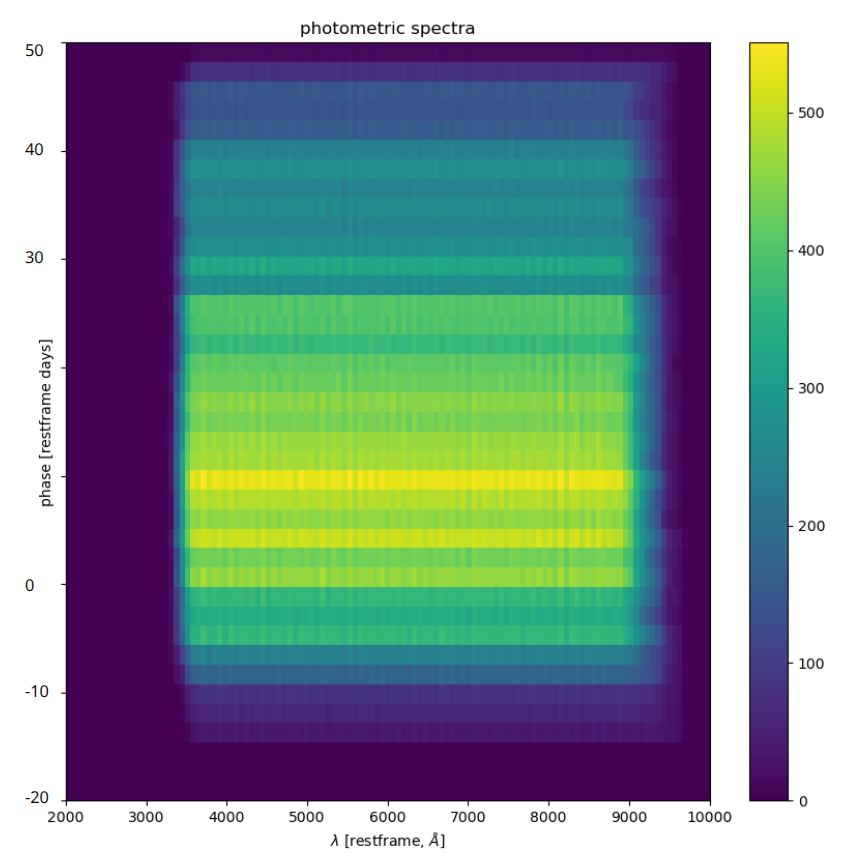
\includegraphics[width=0.7\textwidth]{MainLayout/NaCl_chapter/figures/snfactory/coverage.png}
    \caption{Coverage of the SNfactory data in the $\lambda-p$ space.}
    \label{fig:snf_coverage}
\end{figure}

\subsubsection{Fitting the spectra}

We present in Figure \ref{fig:snf_spectra} examples of spectra that were fitted with NaCl. These are 2 spectra randomly picked out that belong to two different supernova 
and are taken at different phases. What we see is that the trained model seems to accurately describe the evolution of those spectra. The errorsnake model employed 
shows an intrinsic dispersion of the fluxes at an order of about 10\%. We present in the next subsection the results of full dataset.\\

 The entirety of the model training takes around 30 minutes on a Dell Precision 3581 laptop 
equipped with an Intel(R) Core(TM) i7-13700H, 14 cores, up to 5.0 GHz, 32 GB RAM and a NVIDIA RTX A1000 6GB GPU. \\

\begin{figure}[htpb]
\centering
\begin{subfigure}{0.9\textwidth}
    \centering
    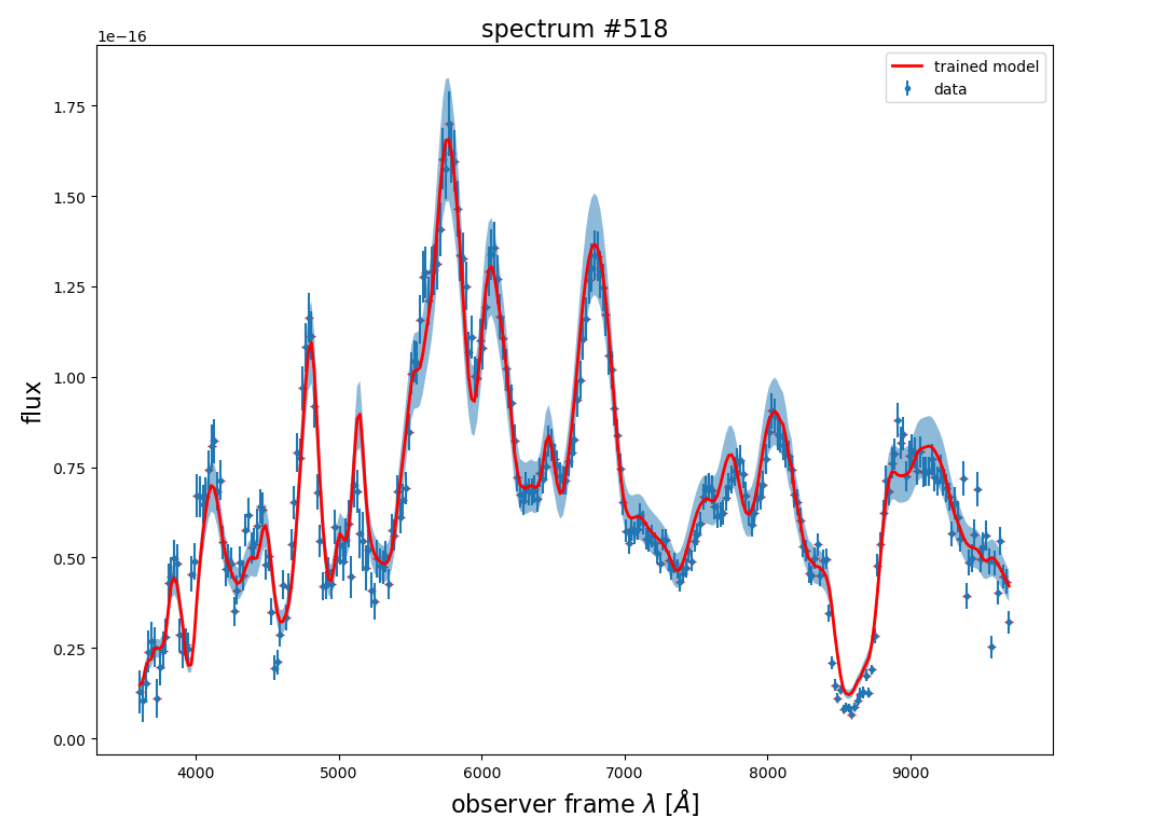
\includegraphics[width=0.9\textwidth]{MainLayout/NaCl_chapter/figures/snfactory/spec_518.png}
    \caption{}
    \label{fig:snf_spec_1}
\end{subfigure}%

\vspace{1em}

\begin{subfigure}{0.9\textwidth}
    \centering
    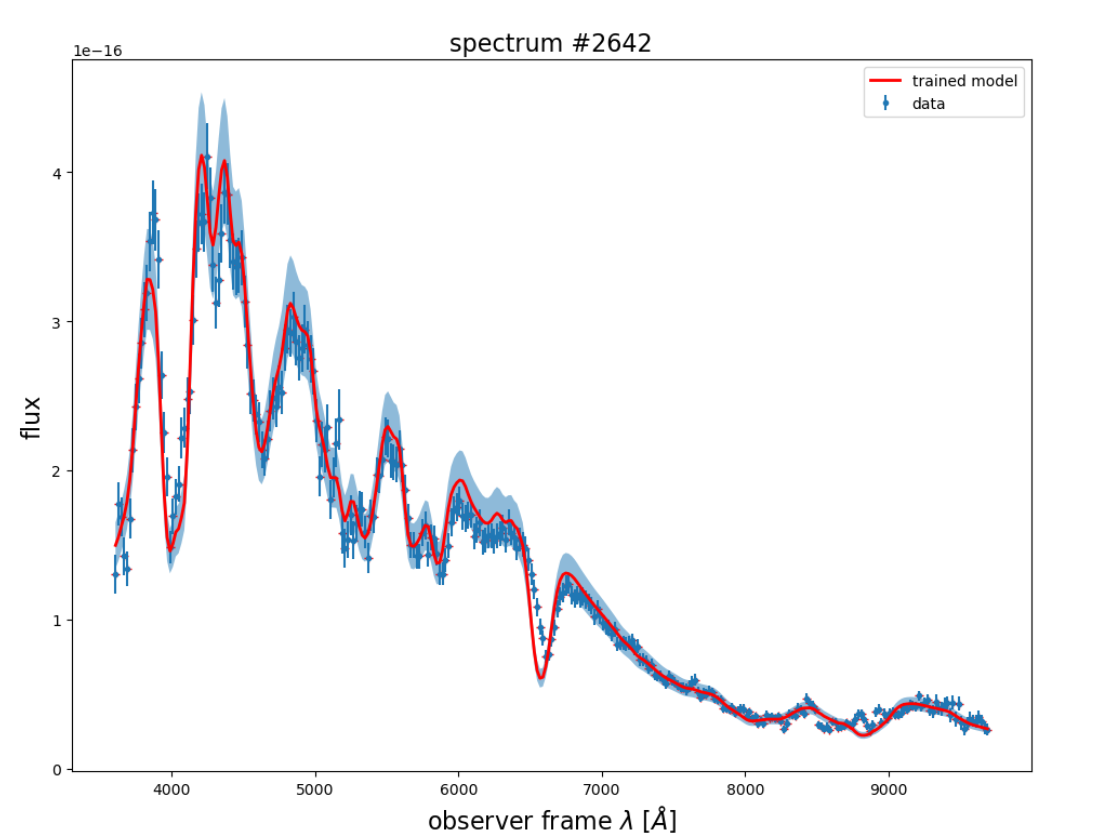
\includegraphics[width=0.9\textwidth]{MainLayout/NaCl_chapter/figures/snfactory/spec_2642.png}
    \caption{}
    \label{fig:snf_spec_2}
\end{subfigure}
\caption{Two spectra with the train NaCl model. The blue points are the data, the red line is the trained model and the highlighted area is the error model.}
\label{fig:snf_spectra}
\end{figure}

\subsubsection{Training residuals}

We would like to examine how well a SALT2 like parameterized model is able to describe the spectrophotometric evolution of supernovae. 
In order to do that, we will be looking at the weighted residuals of the model on the entirety of the data and check if there are any particular features that stand out. 
This is presented in Figure \ref{fig:snf_pulls} where we have calculated the weighted residuals which represent by how many $\sigma$ our model differs from the data, 
also known as pulls. We do that for each data point and stack them on top of each other if they have been observed at the same time. So for example if we have 2 spectra 
measured at phase of $p= -1$ with data points at $5000{\AA}$, it'll appear as one point on the Figure and its value will be the average of the 2 pulls. We then get a 
Figure that represents the accuracy of the model in the $\lambda-p$ space. This also means that each horizontal line represents on average how well a spectrum is modeled 
at that particular restframe phases, while the vertical lines are for specific restframe wavelengths. \\

\noindent We see in the Figure \ref{fig:snf_pulls} that for most of the $\lambda-p$ space the residuals show good agreement between the model and the data. 
But what also stands out is that we can identify three distinct wavelength regions where the model is unable to capture the variability of the data. 
These three regions are found at $\sim 3500 {\AA}$, $\sim 6000 {\AA}$ and $\sim 8000 {\AA}$, which correspond to UV, Si II and Ca II. These are known to 
have very diverse forms (\cite{Wang_2012_UV}, \cite{Parrent_2016_Si_II}) and we can see here that they are not captured by a SALT2 parameterization. 
It is important to mention that the models mentioned in Chapter 2 that go beyond the SALT2 parameterization can capture those variabilities with the help of extra parameters.

\begin{figure}[ht]
    \centering
    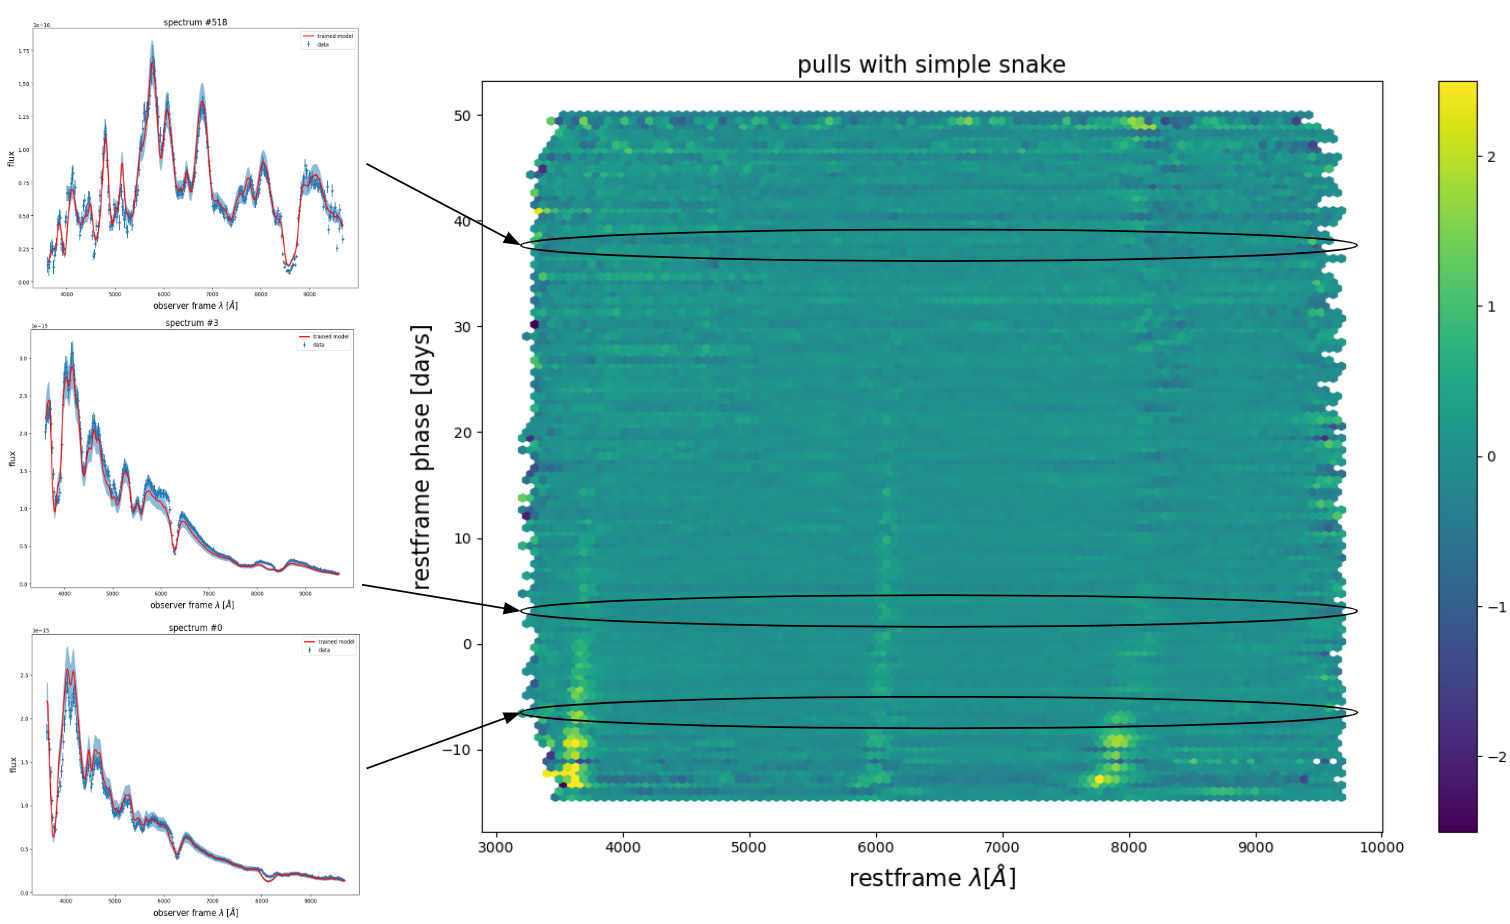
\includegraphics[width=1\textwidth]{MainLayout/NaCl_chapter/figures/snfactory/pulls.png}
    \caption{Weighted residuals at the end of the training done with NaCl on the SNfactory data. The color bar represents by how many $\sigma$ our model differs from the data. We also use as examples 3 spectra at 3 different phases and show where they would be present on the plot.}
    \label{fig:snf_pulls}
\end{figure}

